\documentclass[12pt]{article}
\usepackage{parskip}
\usepackage[letterpaper, margin=1in]{geometry}
\usepackage{graphicx}
\usepackage{subcaption}
\usepackage{amsmath}
\graphicspath{{./images/}}
\title{ELECENG 2EI5 Lab 5}
\author{Raeed Hassan \\ hassam41 \\  \\ McMaster University}
\begin{document}
\maketitle
\pagebreak

\begin{enumerate}
    \item The photograph of the hardware setup is shown in Figure \ref{fig:Circuit}.
    \begin{figure}[h!]
        \centering
        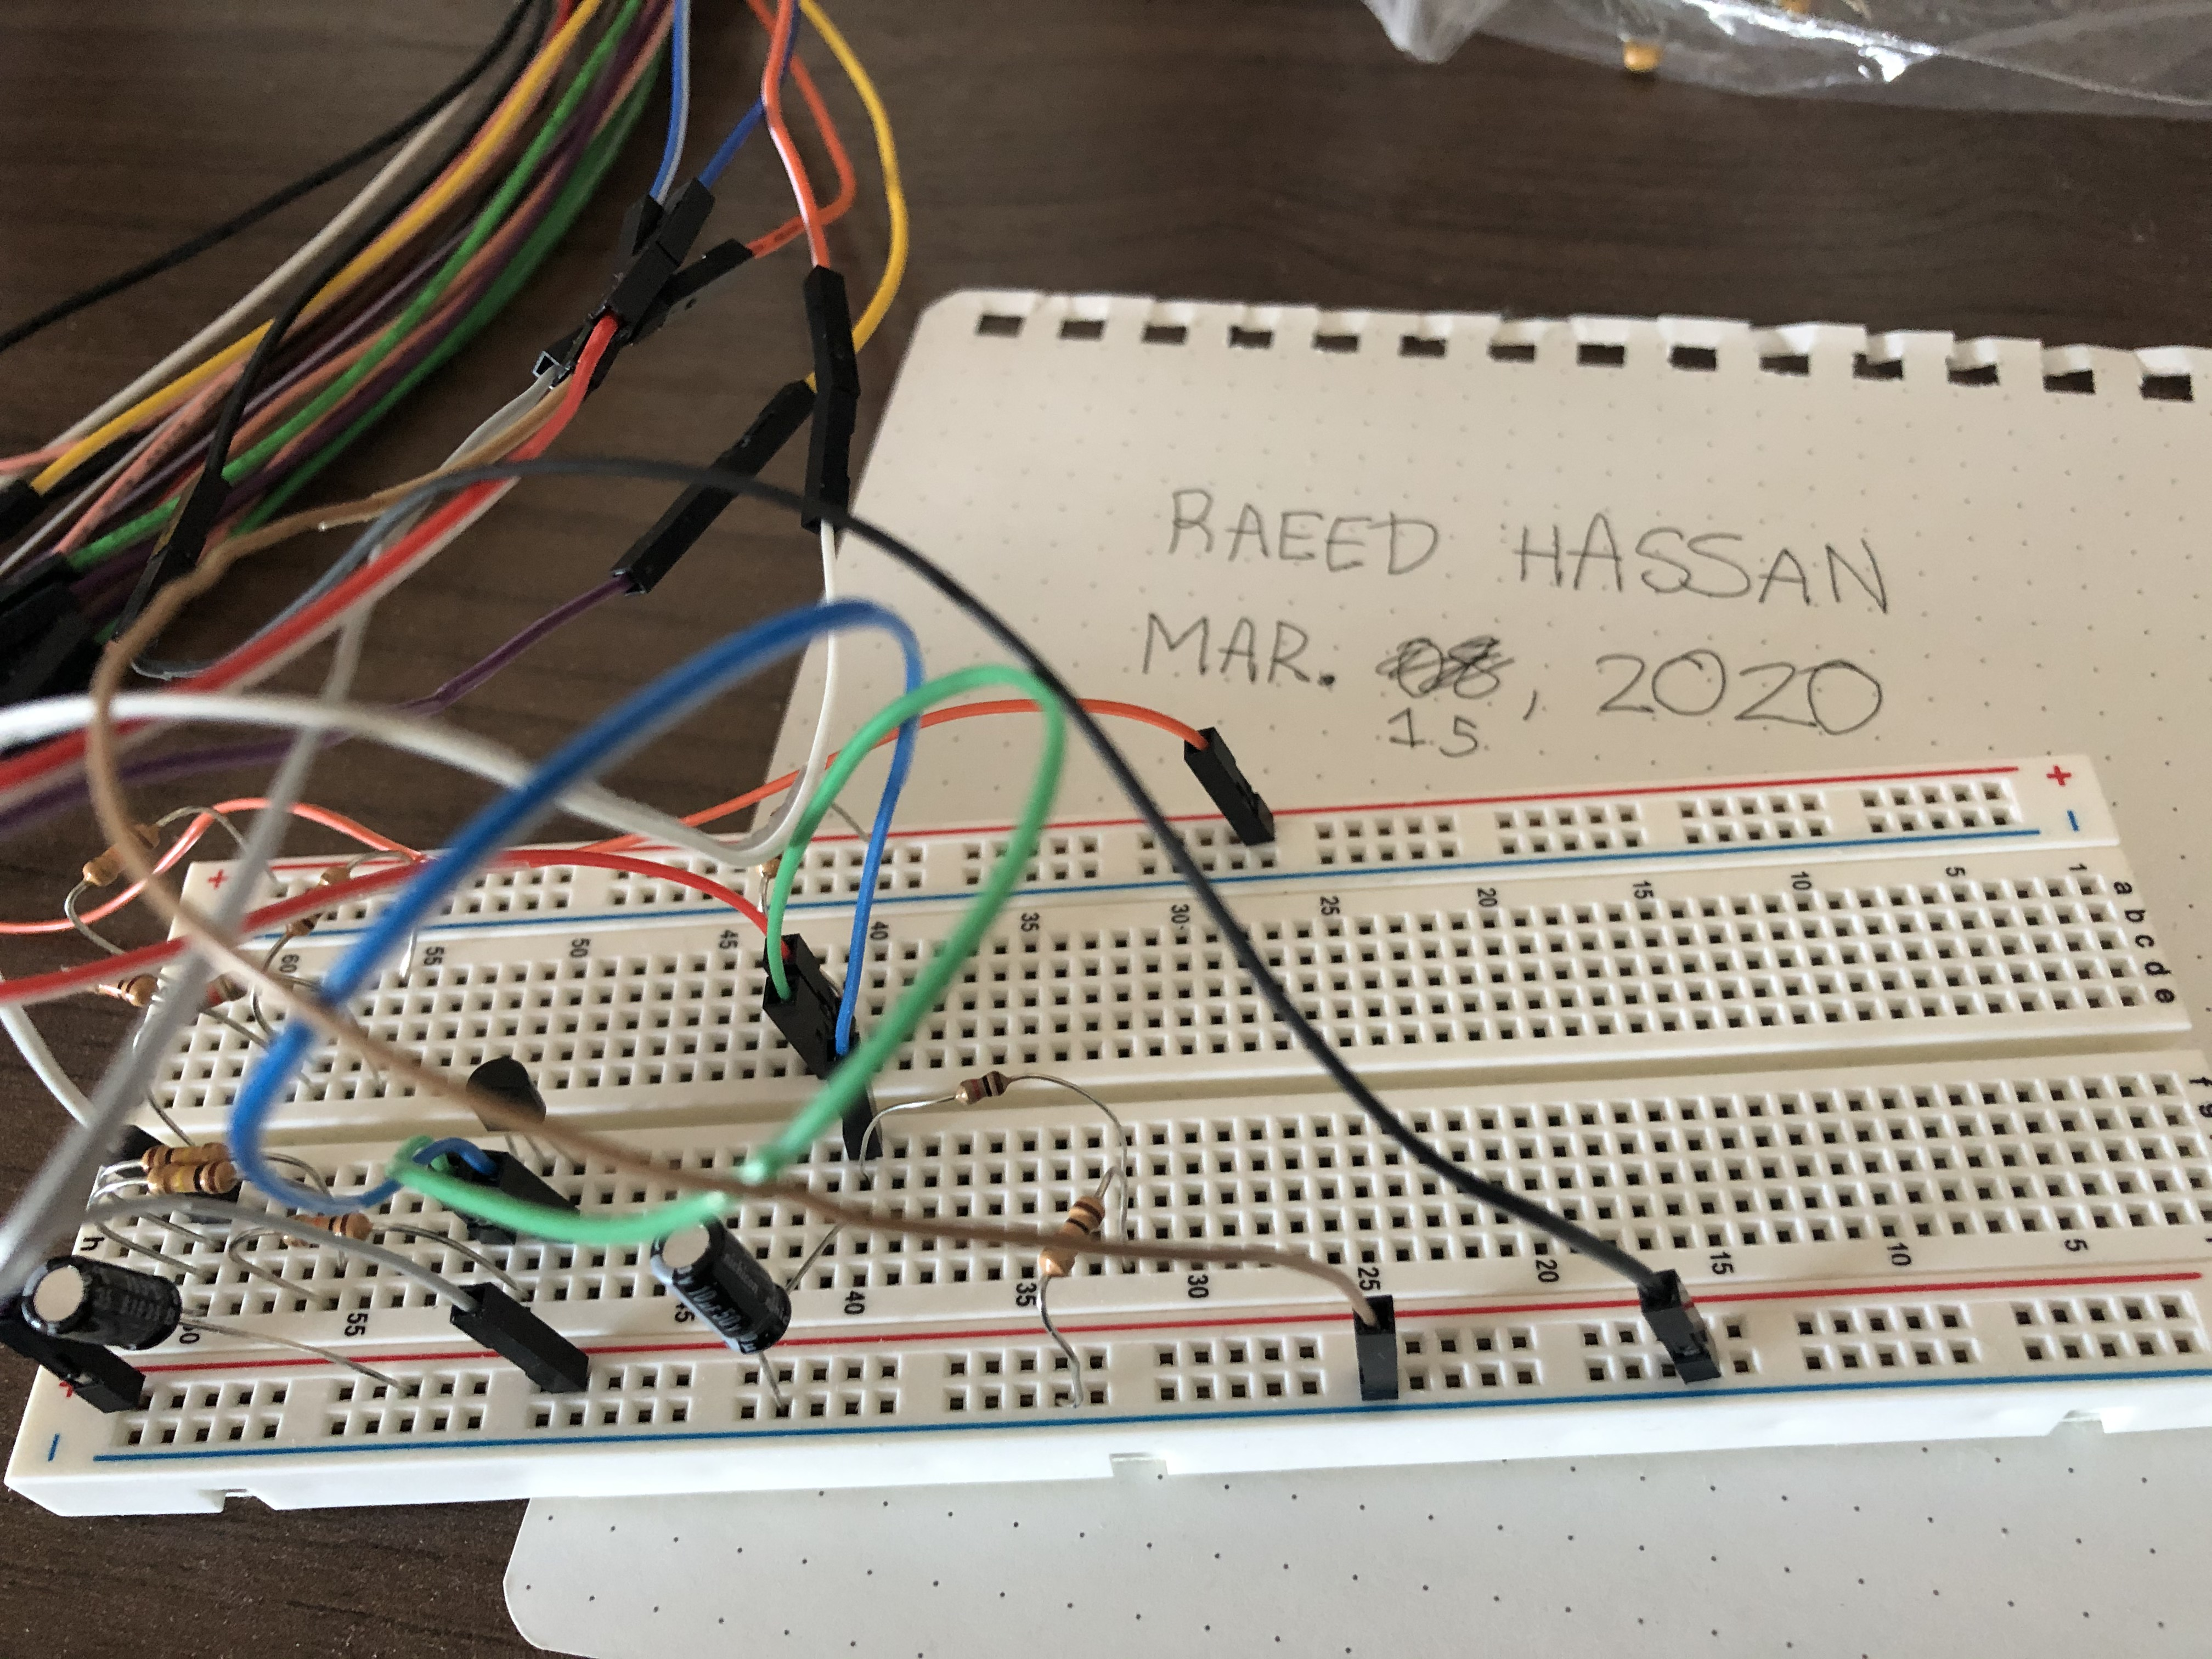
\includegraphics[width=\textwidth]{Circuit.png}
        \caption{Photograph of hardware setup}
        \label{fig:Circuit}
    \end{figure}
    \item Measurements
    \begin{enumerate}
        \item The circuit shown in the lab instructions was built. To measure $v_{in}$, the positive channel of scope 1 was connected to the wavegen 1, and the negative channel of scope 1 was connected to ground. To measure $v_o$, the positive channel of scope 2 was connected to the node connected to the emitter and the $1k\Omega$ resistor, and the negative channel of scope 2 was connected to ground. 
        \item The shape of the output voltage changes when the shape of the input voltage is changed. Examples of this effect can be seen in Figure \ref{fig:MeasurementShapes}. \\
        \begin{figure}[h!]
            \centering
            \begin{subfigure}[b]{0.31\textwidth}
                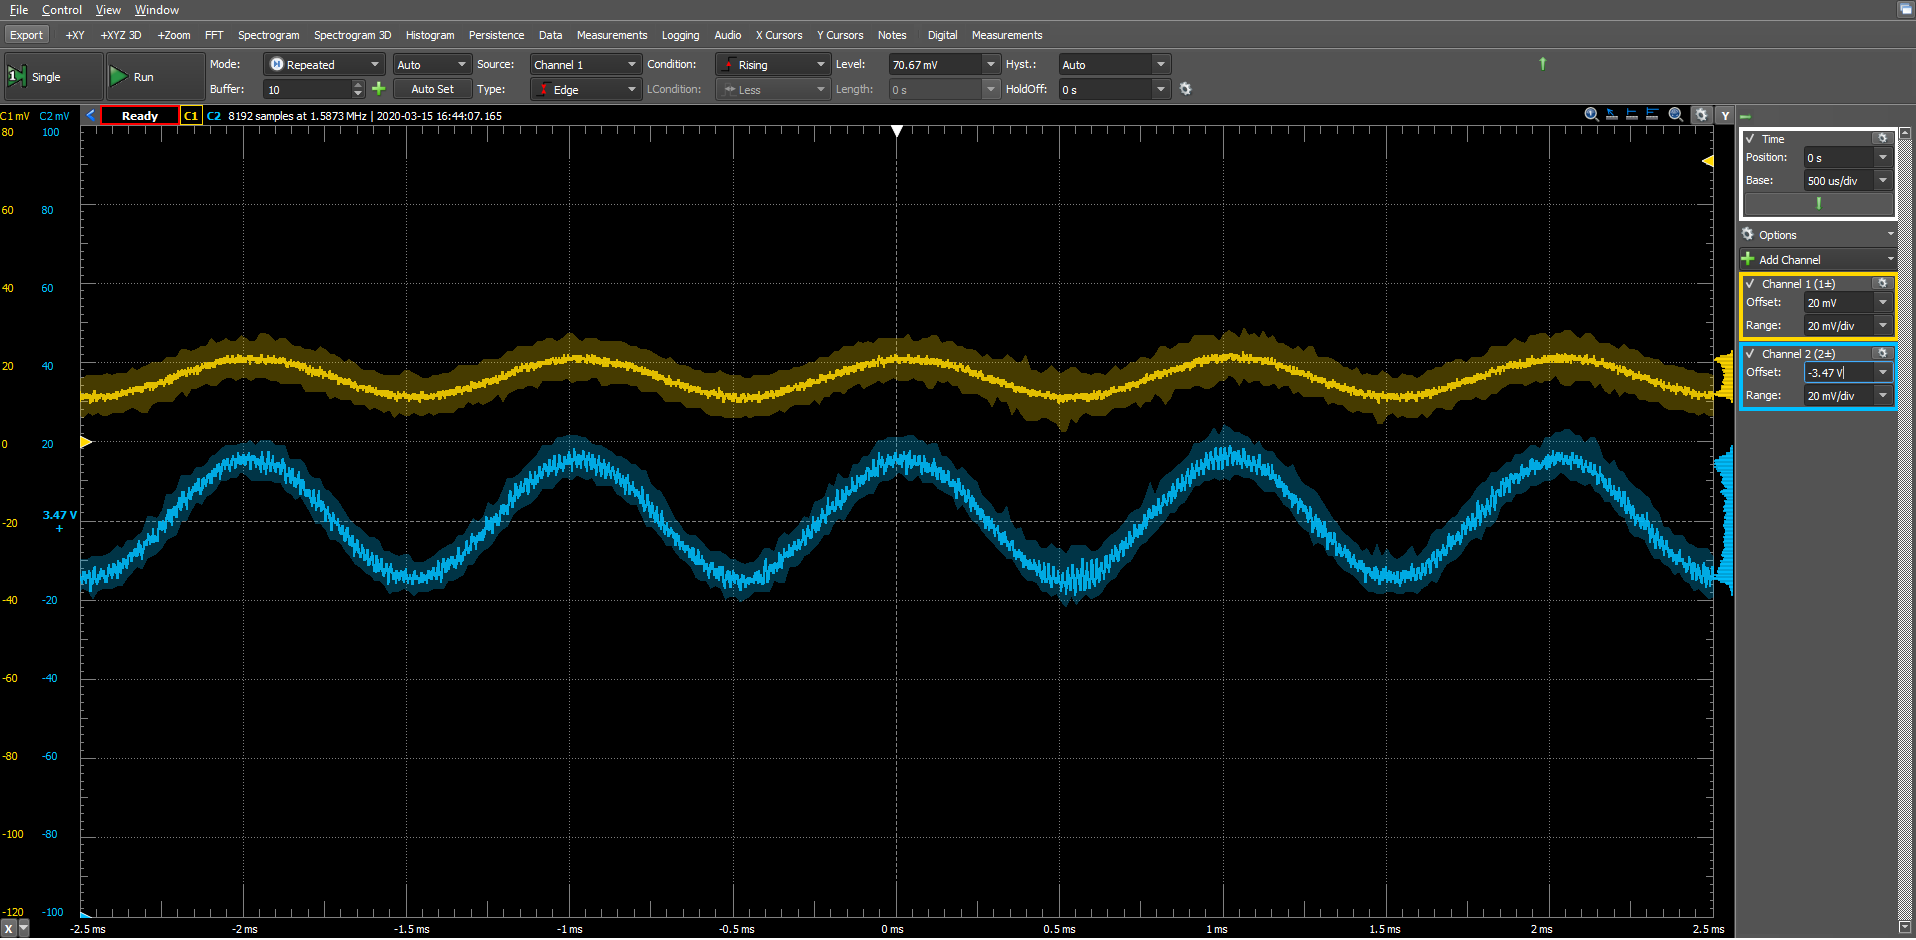
\includegraphics[width=\textwidth]{MeasurementsSine.png}
            \end{subfigure}
            \!
            \begin{subfigure}[b]{0.31\textwidth}
                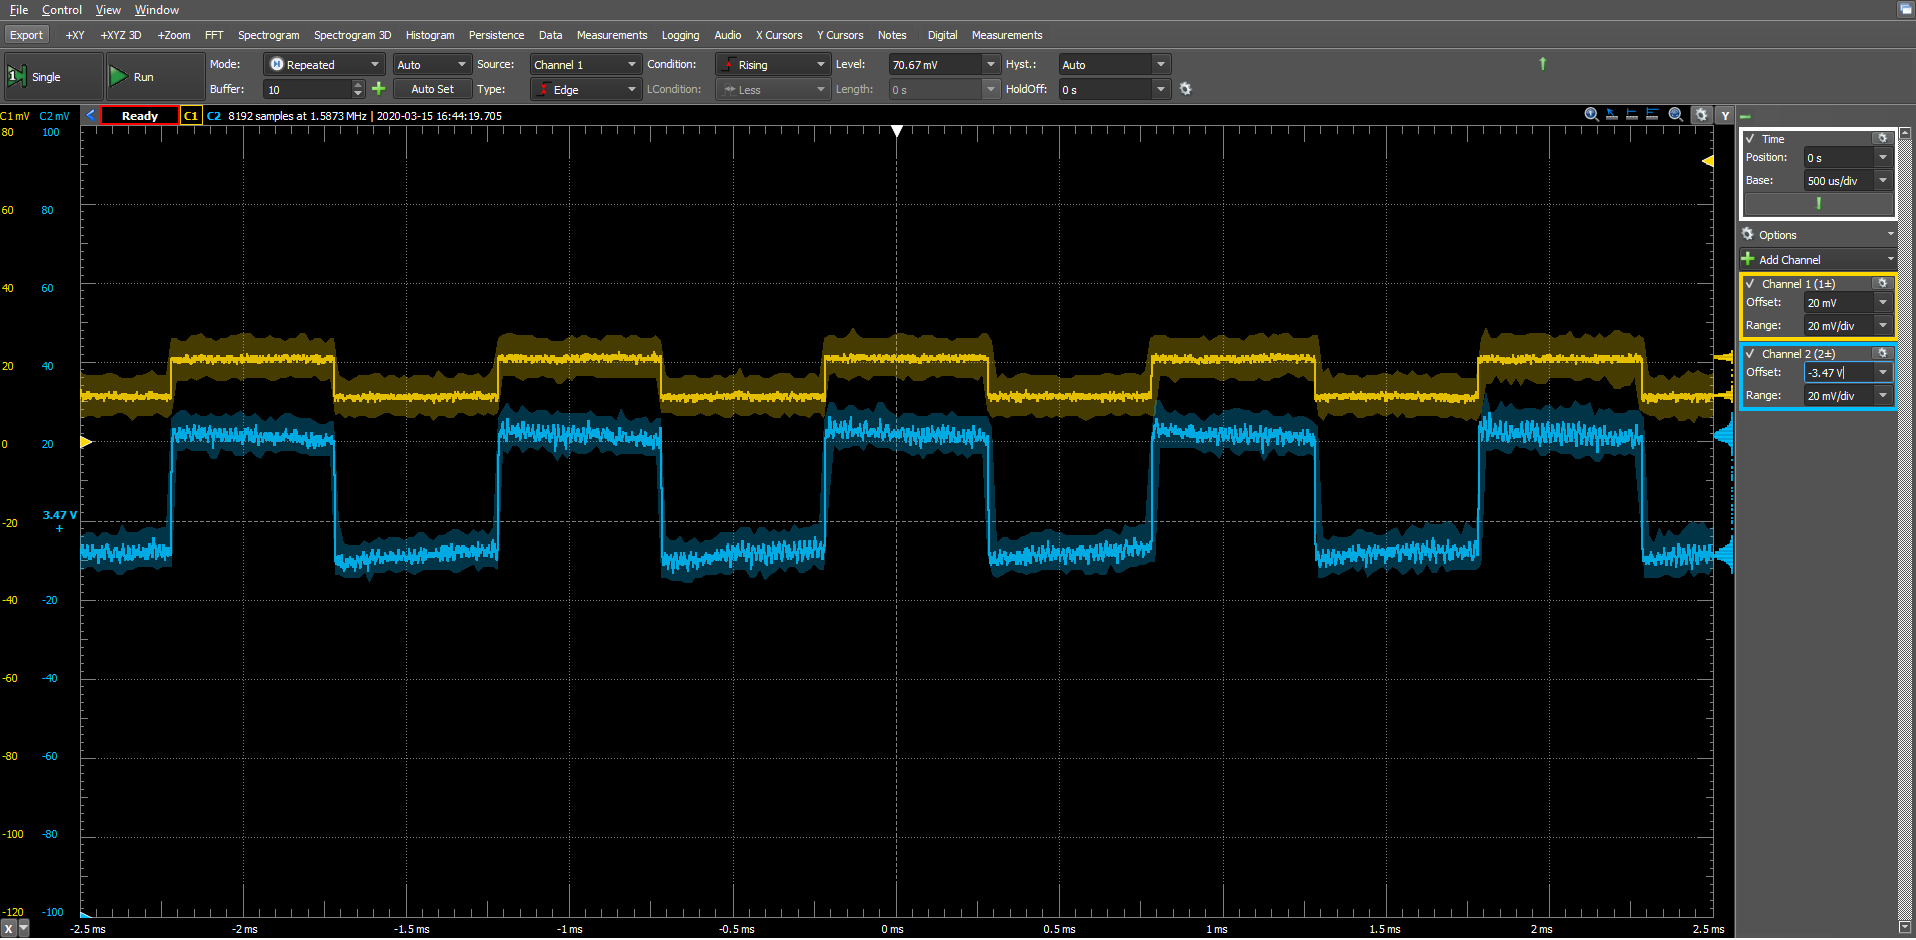
\includegraphics[width=\textwidth]{MeasurementsSquare.png}
            \end{subfigure}
            \!
            \begin{subfigure}[b]{0.31\textwidth}
                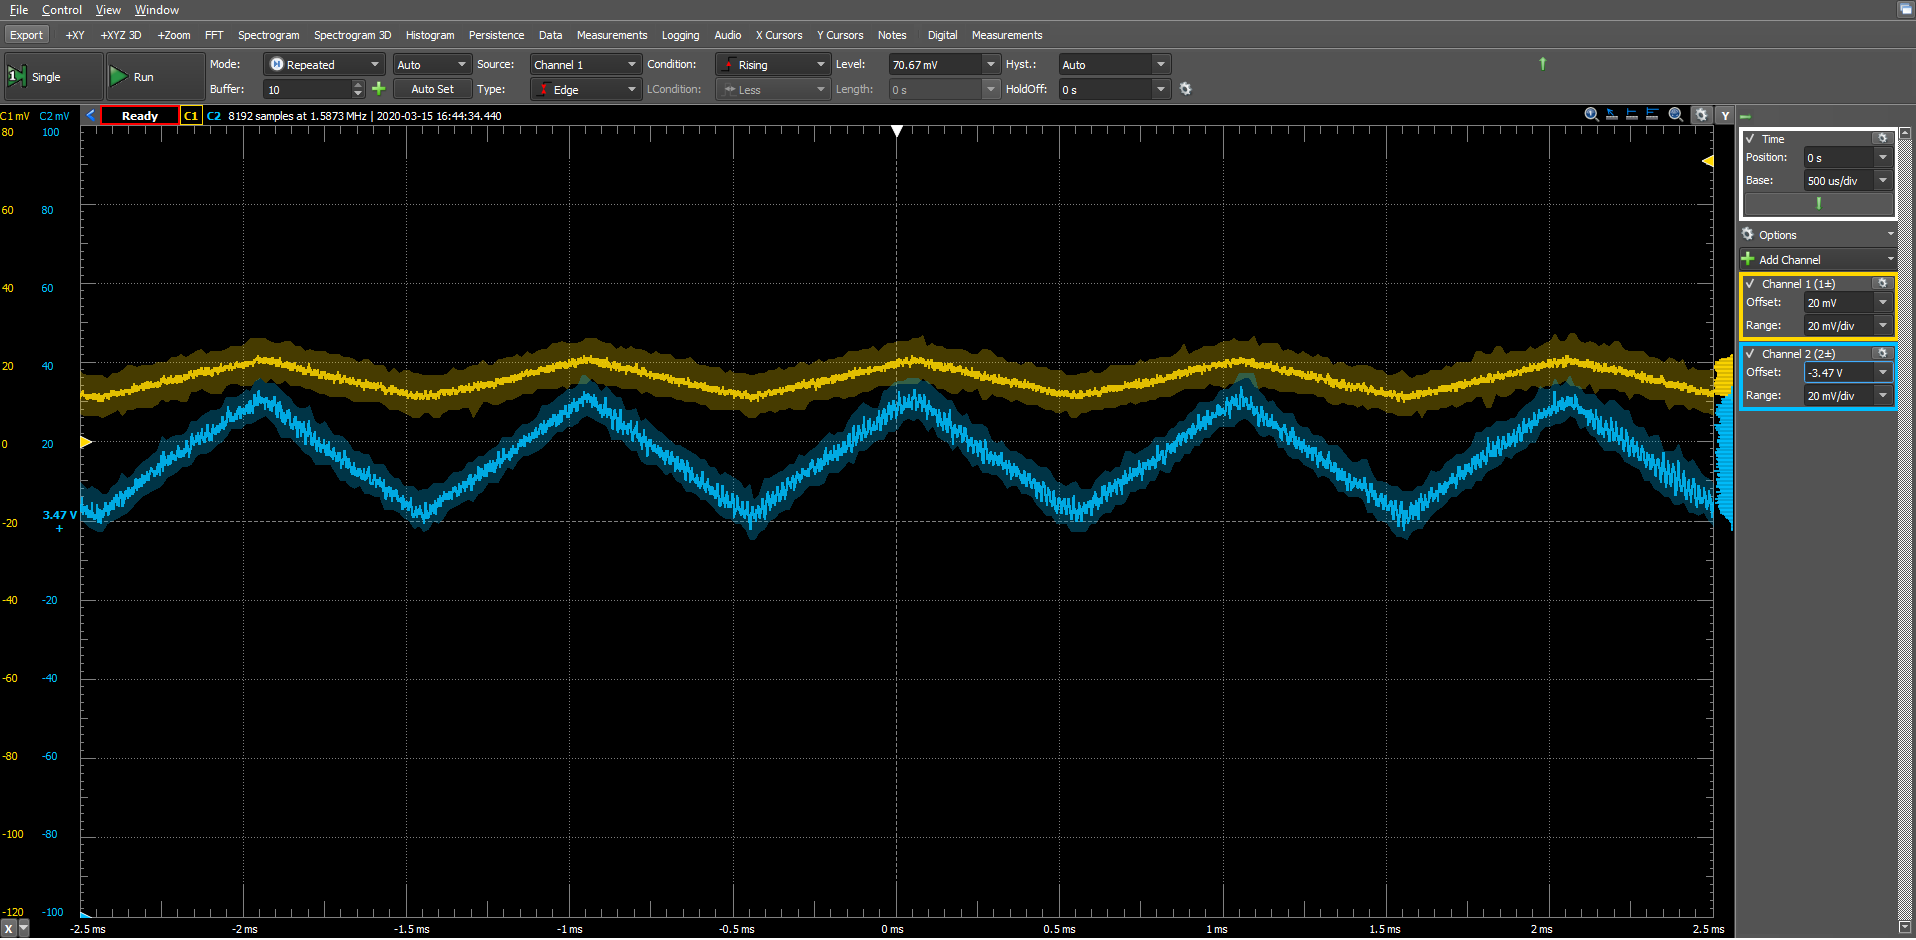
\includegraphics[width=\textwidth]{MeasurementsTriangle.png}
            \end{subfigure}
            \caption{$v_{in}$ (yellow) and $v_o$ (blue) for different input waveforms}
            \label{fig:MeasurementShapes}
        \end{figure} \newpage
        The shape of the graphs do not seem to be affected at very high or very low frequencies, however this is difficult to observe to the large amount of noise present in the graphs. In general, the average voltage values for the output remain similar.

        The DC bias at the input does not have an effect on the output voltage. Changing the AC amplitude of the input changes the AC amplitude at the output, increasing if the input amplitude is increase and decreasing if the input amplitude is decreased, and eventually begins to distort the shape of the output if it is increased enough.
    \end{enumerate} \newpage
    \item Simulations
    \begin{enumerate}
        \item The schematic capture of the circuit can be seen in Figure \ref{fig:Schematic}. \\
        \begin{figure}[h!]
            \centering
            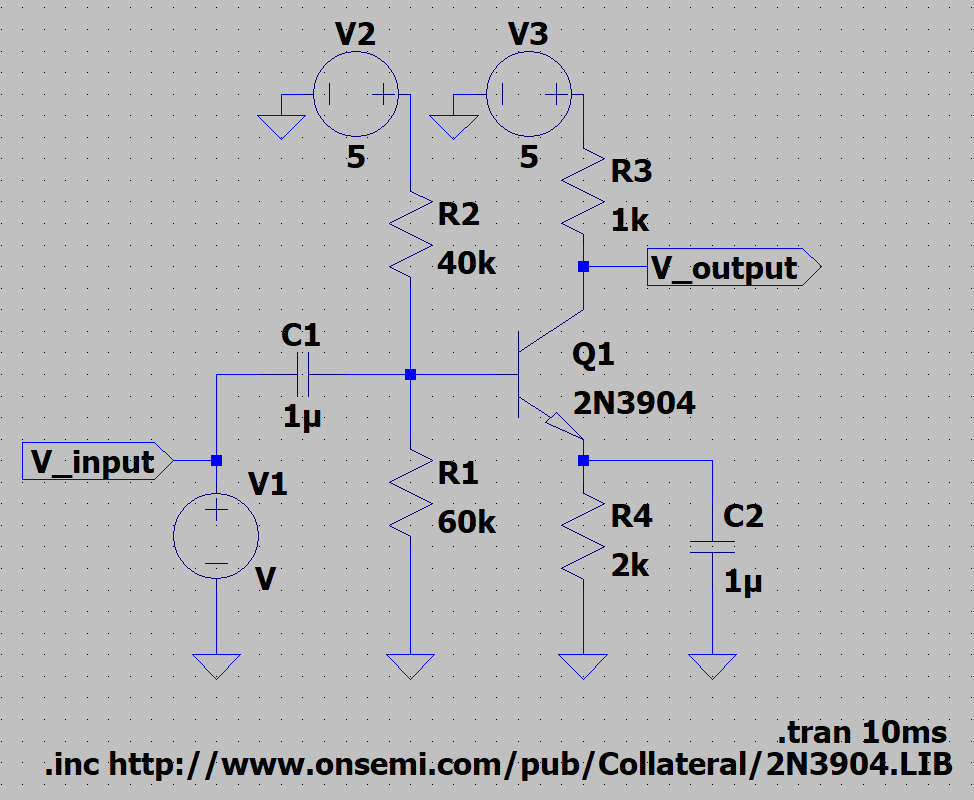
\includegraphics[width=\textwidth]{Schematic.png}
            \caption{The schematic of the circuit}
            \label{fig:Schematic}
        \end{figure} \\
        \item The netlist for the simulation can be seen in Figure \ref{fig:Netlist}. The model used for NPN is provided by the manufacturer of the NPN used in the circuit built in the experimental portion of the lab.
        \begin{figure}[h!]
            \centering
            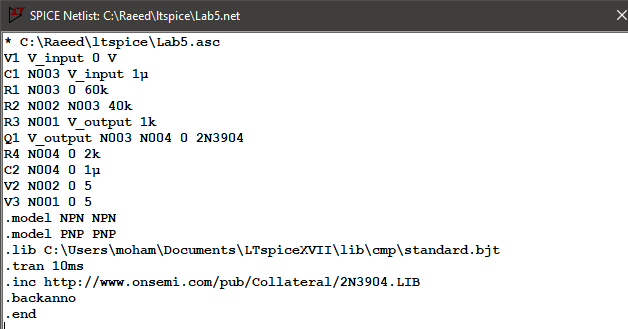
\includegraphics[width=\textwidth]{Netlist.png}
            \caption{The netlist of the simulation}
            \label{fig:Netlist}
        \end{figure} \newpage
        \item The shape of the output voltage changes when the shape of the input voltage is changed. Examples of this effect can be seen in Figure \ref{fig:SimShapes}. \\
        \begin{figure}[h!]
            \centering
            \begin{subfigure}[b]{0.31\textwidth}
                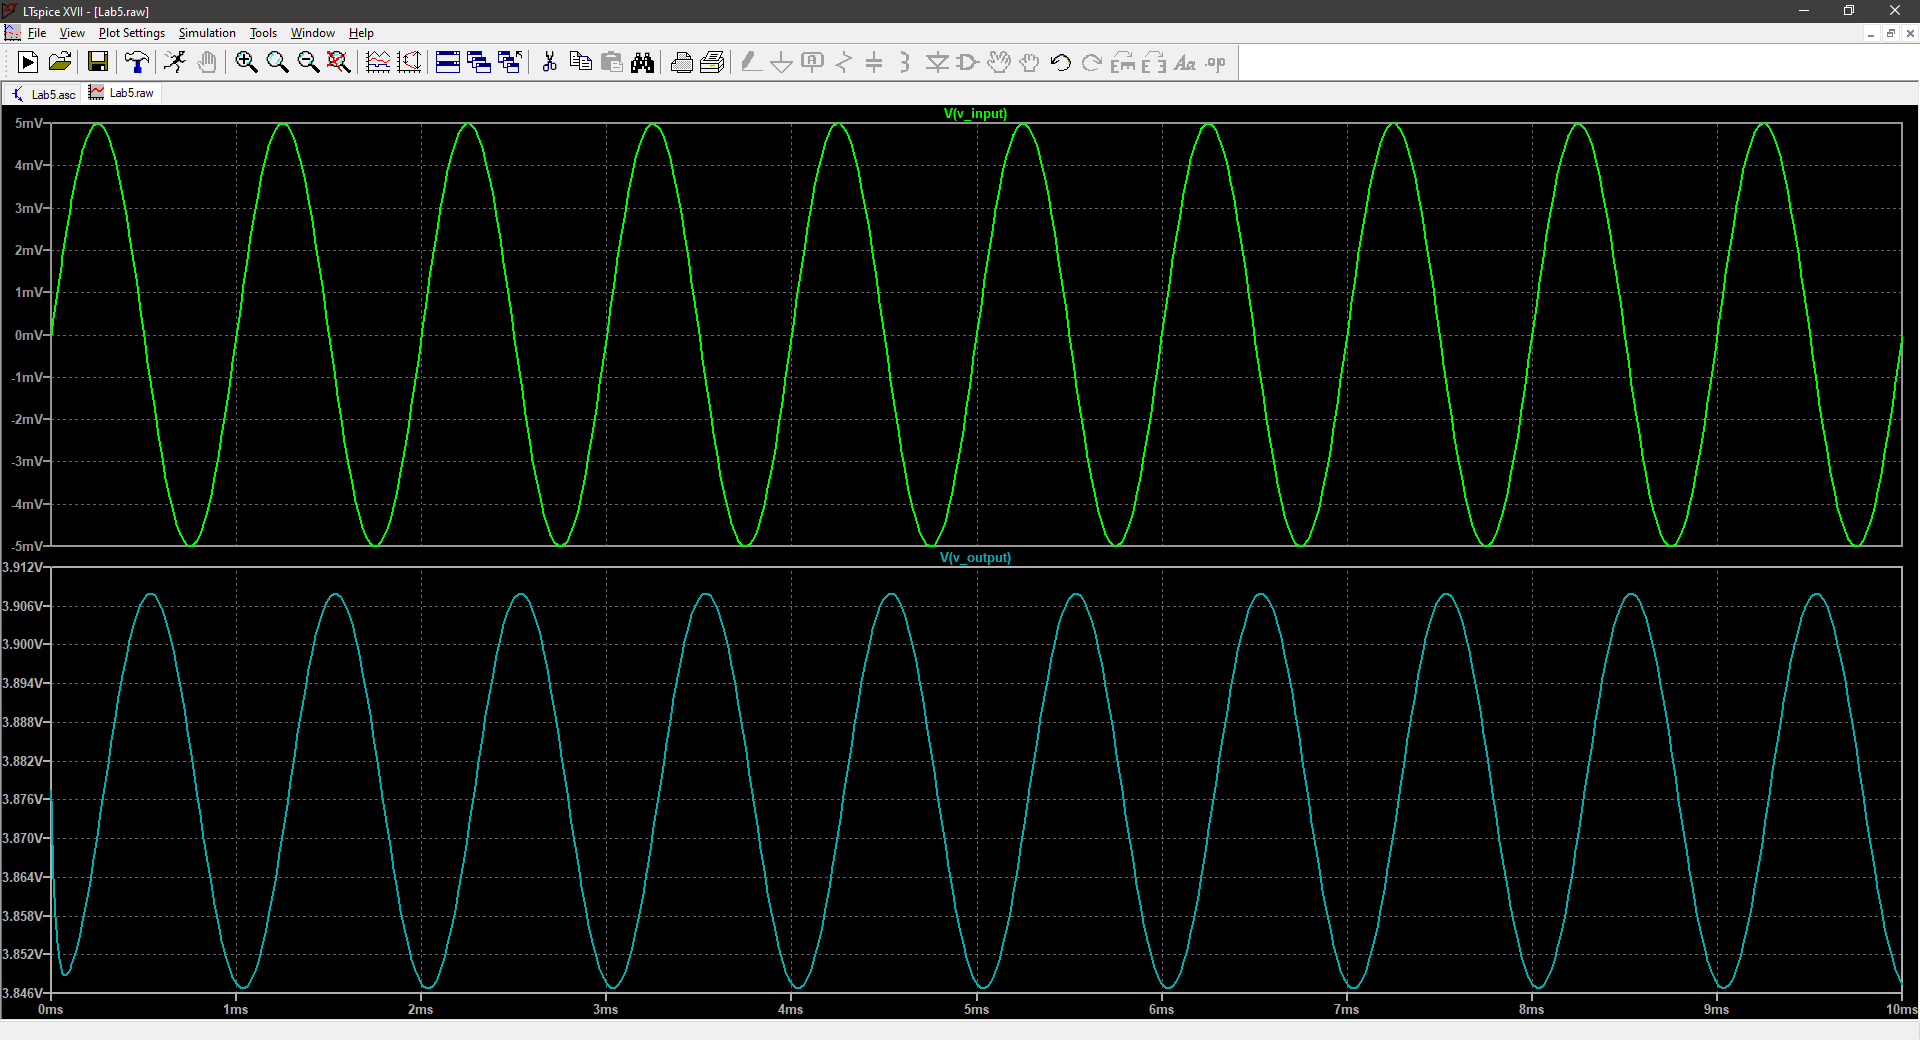
\includegraphics[width=\textwidth]{SchematicSine.png}
            \end{subfigure}
            \!
            \begin{subfigure}[b]{0.31\textwidth}
                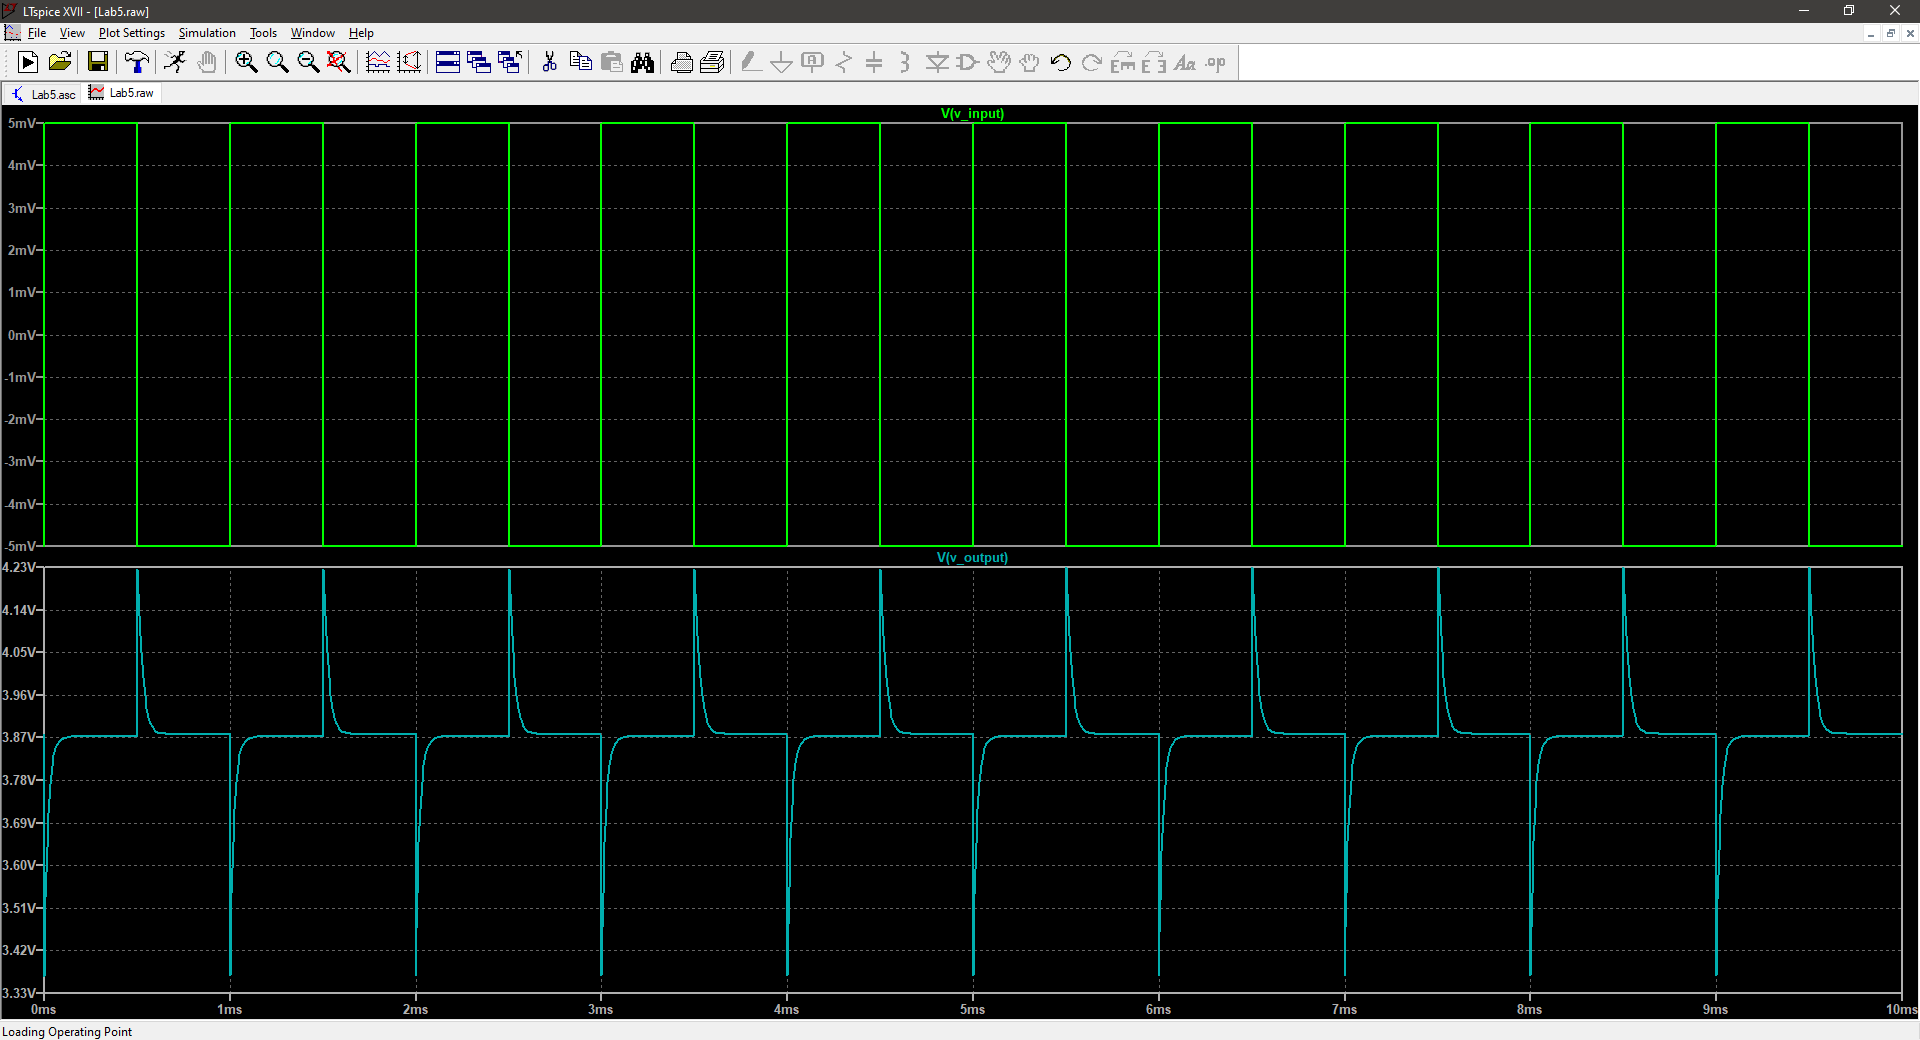
\includegraphics[width=\textwidth]{SchematicSquare.png}
            \end{subfigure}
            \!
            \begin{subfigure}[b]{0.31\textwidth}
                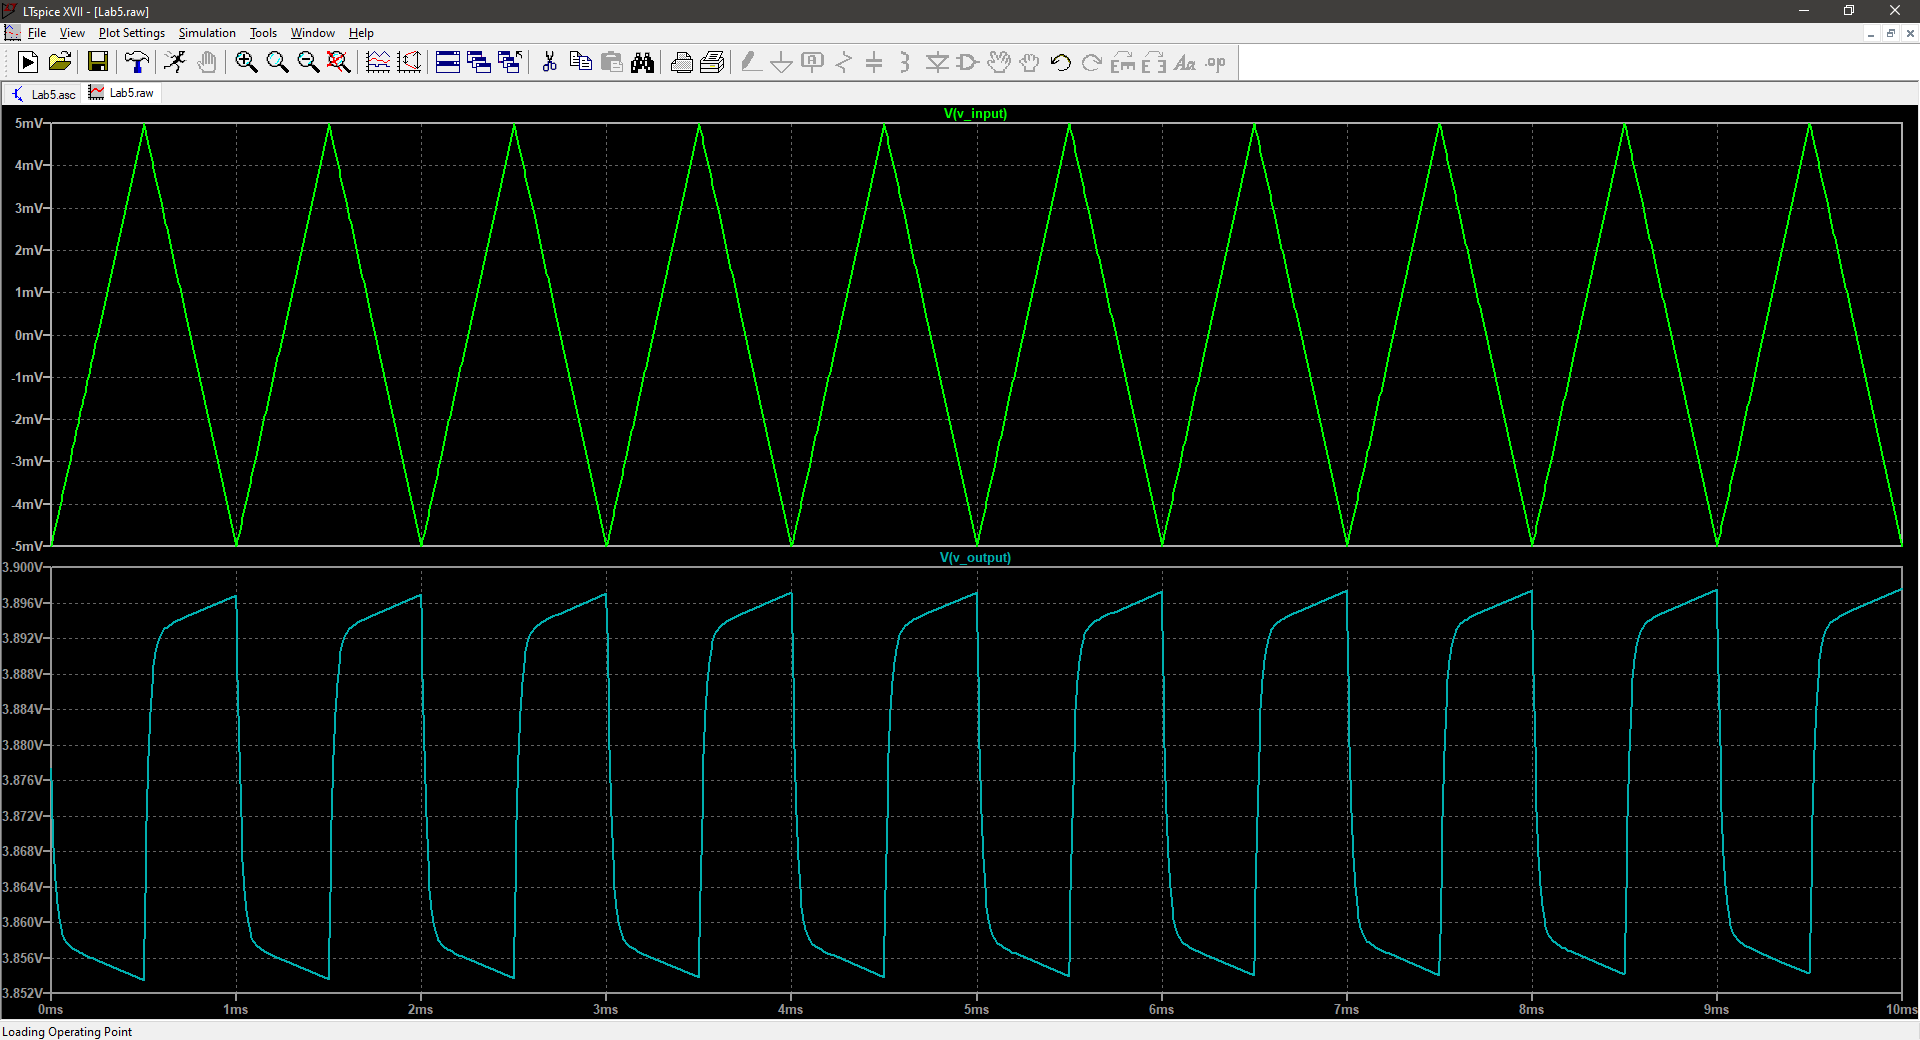
\includegraphics[width=\textwidth]{SchematicTriangle.png}
            \end{subfigure}
            \caption{$v_{in}$ (green) and $v_o$ (cyan) for different input waveforms}
            \label{fig:SimShapes}
        \end{figure} \\
        The shape of the graph after some time does not seem very affected by the frequency of the input except the initial time it takes for the output to stabilize (which is being affected both by the frequency of the input and the changing time constant caused by this change in frequency). The average value of the output remains similar regardless of the frequency, with the only change being in the amplitude of the output. At very low frequencies, the amplitude of the output becomes very small. The amplitude increases with increasing frequency, however this is only up to a certain point. At around 100 MHz, the amplitude of the output begins to decrease, however it does not reach extremely small values like at very small frequencies.
        
        The DC bias at the input does not have an effect on the output voltage. Changing the AC amplitude of the input changes the AC amplitude at the output, increasing if the input amplitude is increase and decreasing if the input amplitude is decreased, eventually begins to distort the shape of the output if it is increased enough. This effect can be seen in Figure \ref{fig:SimACDist}.
        \begin{figure}[h!]
            \centering
            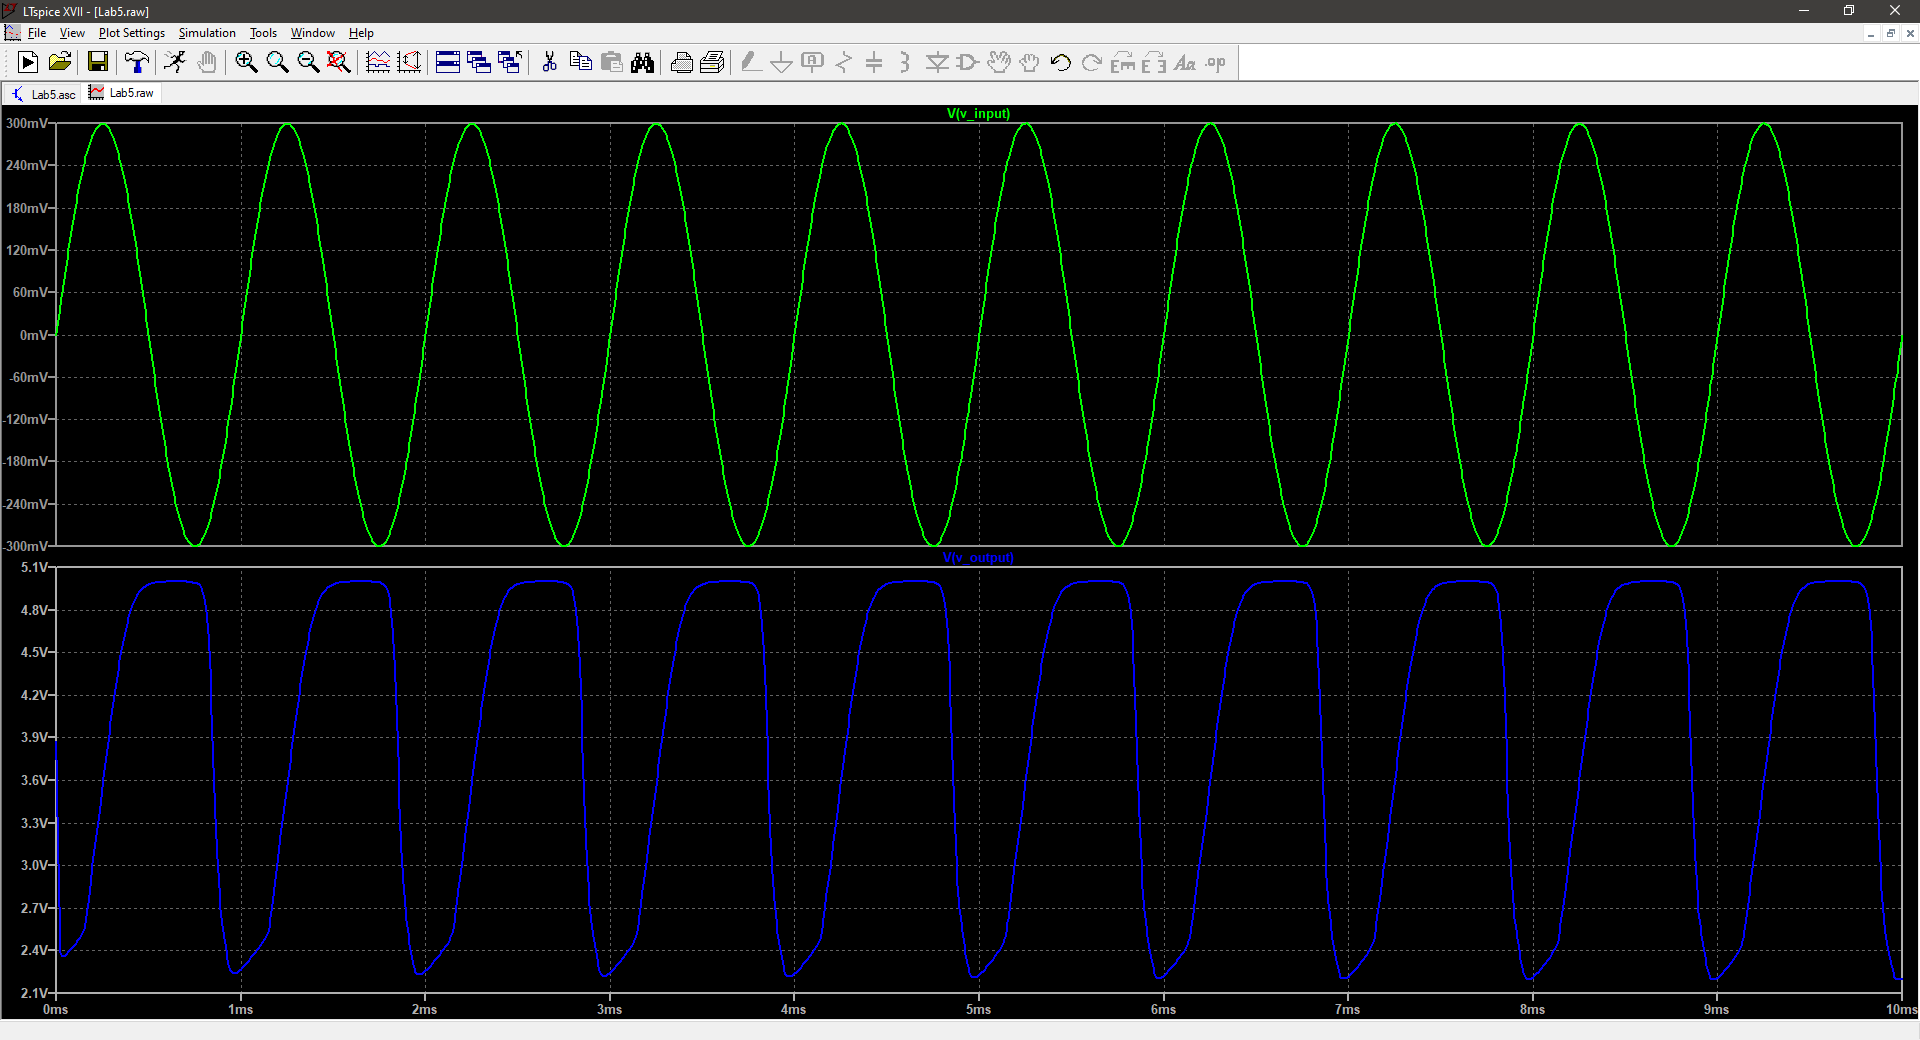
\includegraphics[width=\textwidth]{SchematicACDistortion}
            \caption{Distortion in output when AC ampltiude of input is increased}
            \label{fig:SimACDist}
        \end{figure}

        Removing capacitors from the circuit would affect the circuits ability to filter the DC bias present at the input, and in the current circuit setup, affect the the NPN's ability to operate. Removing both capacitors causes the output voltage to remain static at $5V$. Removing the capacitor at the input causes the average voltage at the output to be $5V$, with the amplitude of the output being affected by the remaining capacitor. Removing the capacitor at the emitter of the NPN will not affect the average voltage at the output, but will affect the amplitude of the output voltage.
        
        Changing resistance values will simply affect the gain of the circuit depending on which resistor values are changed.  
    \end{enumerate}
    \item There were major discrepanies between the simulations and experimental data, particularly in the amplitude and average voltage at the output. In experiments, the average amplitude was significantly lower than the simulated amounts, and the average voltage was also slightly lower. 
    \item There were some issues caused by the AD2 board when performing experiments. For example, even when the DC bias of the input waveform was set to zero, the scope would always display a DC bias at the input, and its amplitude would be significantly higher as well, almost double when it was set to $10 mV$ peak to peak.
\end{enumerate}
\end{document}
